\documentclass[11pt,letterpaper]{article}

%\usepackage{times}
%\usepackage{epsfig}
\usepackage{graphicx}
%\usepackage{amsmath}
%\usepackage{amssymb}
\usepackage{hyperref}
\usepackage{tabularx}
\usepackage[left=1in, right=1in, top=1in, bottom=1in]{geometry}
\usepackage{titling}
\usepackage{setspace}
\usepackage{sectsty}
\usepackage{tabto}
\graphicspath{{./Assignment_01_Geidel_files/}} % adds the assets directory to the path, throw your images there
\usepackage{fancyhdr}
\pagestyle{fancy}
\fancyhf{}
\fancyheadoffset{0cm}
\renewcommand{\headrulewidth}{0pt} 
\renewcommand{\footrulewidth}{0pt}
\fancyhead[R]{\thepage}
\fancypagestyle{plain}{%
  \fancyhf{}%
  \fancyhead[R]{\thepage}%
}

\usepackage{cite}
\usepackage[sectionbib]{natbib}
\renewcommand{\refname}{}

\begin{document}
\fontfamily{ptm}\selectfont
\sectionfont{\fontsize{12}{12}\fontfamily{ptm}\selectfont}
\doublespacing
%%%%%%%%%%%%%%%%%%%%%%%%%%%%%% TITLE %%%%%%%%%%%%%%%%%%%%%%%%%%%%%%%%%%%%%%
\setlength{\droptitle}{1in} 

\title{\large{ASSIGNMENT 1: \\ FINANCIAL PLANNING AGENT \\\vspace{1.2in}}}

\author{
Kevin Geidel \\
MSDS 442: AI Agent Design \& Development \\
Northwestern University \\
May 4, 2025 \\
}

\date{}
\maketitle
\thispagestyle{empty}	
\clearpage
\setcounter{page}{1}

%%%%%%%%%%%%%%%%%%%%%%%%%%%%%% PAGE 1 %%%%%%%%%%%%%%%%%%%%%%%%%%%%%%%%%%%%

\section*{Requirement 1: Graph the Agent with LangChain/LangGraph}
\tab The construction of the agent and accompanying graph begins in cell 2 (see appendix). 
The actual assembly of the graph occurs in cell 7. However, some of the components, such as the retriever \textbf{ToolNode} and \textbf{AgentState} class,
are built above. Following the logic in cell 7 we first instantiate an empty graph:

\begin{verbatim}
workflow = StateGraph(AgentState)
\end{verbatim}

The \texttt{workflow} object has \texttt{add\_node} and \texttt{add\_edge} methods that allow us to assemble the 
components created in cells 2-6. The output is displayed graphically in cell 8 (reproduced below.)
\begin{center}
    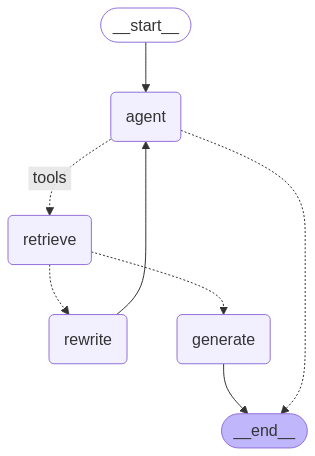
\includegraphics[height=400pt]{Assignment_01_Geidel_7_0.png}
\end{center}

\clearpage

\section*{Requirement 2: Load the Fidelity web pages}
\tab Loading the web pages occurs in in cell 2. A list of URLs are defined and based to the \textbf{WebBaseLoader}.
The \textbf{RecursiveCharacterTextSplitter} chunks the documents into workable pieces. The result is a list of LangChain documents that each have
a portion of each site. The output is sampled below.

\begin{center}
    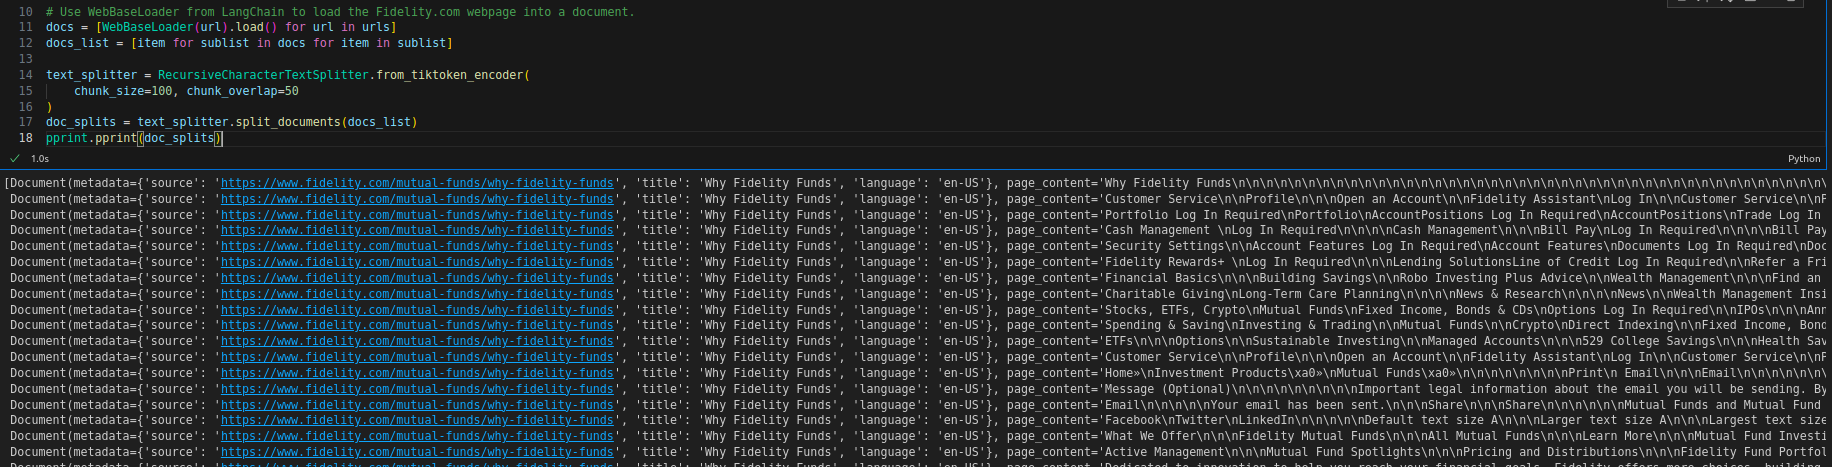
\includegraphics{req_2.png}
\end{center}

\section*{Requirement 3: Store documents in ChromaDB}
\tab The documents are turned into vector embeddings and store in the ChromaDB vector store. This happens in cell 3. 
The embedding model used is \textbf{OpenAIEmbeddings}. The result is a collection of vectors with id's for use in retrieval.

\begin{center}
    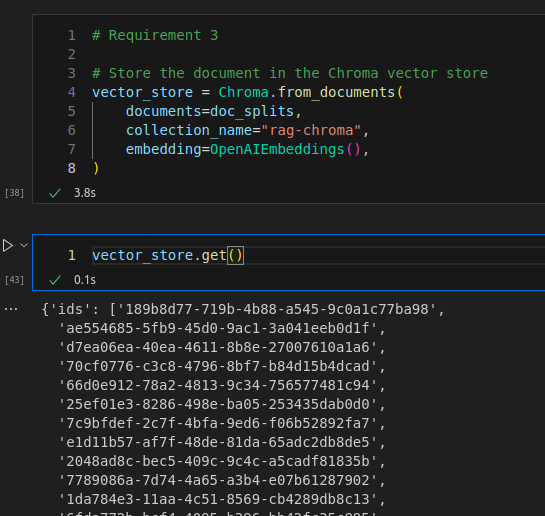
\includegraphics[height=300pt]{req_3.png}
\end{center}

\section*{Requirement 4: Retriever tool for relevance analysis}
\tab In cell 4 the retriever tool that will be used by the AI Agent to verify that the document is relevant to the question asked is created.
The vector store has an \texttt{as\_retriever} method. The tool is created from the retriever and labeled so the agent will know when to use it.
The output is shown as the output of cell 4.

\section*{Requirement 5: Create a chain to determine relevance of question}
\tab Using the agent assembled in cell 7 we prepare to use the chain to evaluate if a question is relevant to the bot's function and knowledge base.
The prompt is constructed in cell 6 in the \texttt{grade\_documents} action. The system message is built from the prompt, which informs the 
LLM it is a financial advisor and spells out how the session will proceed. The output for cell 6 shows the rag prompt ready to be deployed.

\section*{Requirement 6: Prompt the graph}
\tab In cell 9 I construct a function, \texttt{query\_agent}, that passes the user's message to the graph in a \texttt{HumanMessage} along with the system prompt. This allows use to query the agent in a DRY fashion. The prompt for requirement 6, \textit{`What are the steps that I should take to determine how much I need to save for retirement planning'}, yielded the following response:

\begin{verbatim}
{ 'messages': [ "To maintain your preretirement lifestyle in retirement, it's "
                'generally recommended to save 10 times your preretirement '
                'income by age 67. This goal is based on the assumption of '
                'saving 15% of your income annually starting at age 25. '
                'Age-based milestones suggest aiming for 1x your income by age '
                '30, 3x by age 40, and 6x by age 50 to stay on track.'
            ]
}
\end{verbatim}
(To see the full trace, including the steps followed by the agent, see the output of cell 10.)

\clearpage

\section*{Requirement 7: Inspect and evaluate response}
\tab I am not a financial planner but this advice seems sound. The agent recommends a 
decision tree that can be used to determine a quantitative answer for the question
"How much do I need to retire?" In addition to providing the overall method for finding the 
answer to the question it expands by suggesting milestones that align with the answer.

\section*{Requirement 8: A similar prompt}
\tab Another prompt with similar semantic meaning is \textit{`What strategies should someone take when behind on their retirement milestones?'}.
When queried, the agent gave the following response:

\begin{small}
\begin{verbatim}
AIMessage(content="I can help with questions related to Fidelity 
mutual funds and retirement planning. If you're looking for strategies to catch up 
on retirement milestones, here are some general tips:\n\n
1. **Assess Your Current Situation**: Take a close look at your current savings, 
investments, and retirement accounts. Understand how much you have saved and how 
much you need to retire comfortably.\n\n2. **Increase Contributions**: If possible, 
increase your contributions to retirement accounts. Consider maxing out contributions 
to employer-sponsored plans like a 401(k) or an IRA.\n\n
3. **Catch-Up Contributions**: If you are age 50 or older, take advantage of catch-up 
contributions that allow you to contribute more to your retirement accounts.\n\n
4. **Create a Budget**: Review your expenses and create a budget that allows you to 
allocate more funds toward retirement savings. Cut unnecessary expenses where possible.
5. **Consider Additional Income Sources**: Look for ways to increase your income, such 
as taking on a part-time job, freelancing, or selling unused items.\n\n
6. **Invest Wisely**: Ensure that your investments are aligned with your retirement goals. 
Consider a diversified portfolio that balances risk and growth potential.\n\n
7. **Delay Retirement**: If feasible, consider delaying your retirement age. Working 
longer can increase your savings and reduce the number of years you need to draw 
from your retirement funds.\n\n8. **Consult a Financial Advisor**: A financial advisor 
can provide personalized advice based on your specific situation and help you 
create a plan to get back on track.\n\nIf you have specific questions about Fidelity
 mutual funds or retirement planning, feel free to ask!", 
 additional_kwargs={}, response_metadata={
    'finish_reason': 'stop', 'model_name': 'gpt-4o-mini-2024-07-18', 
    'system_fingerprint': 'fp_129a36352a'
    }, id='run-47220c96-088b-4719-8764-1b241a224edf-0')
\end{verbatim}
\end{small}

This response provides some specific steps for catching up with retirement milestones!

\section*{Requirement 9: Irrelevant prompt}
\tab When passed a prompt that is not relevant to the knowledge base documents the agent responded accordingly.

\begin{center}
    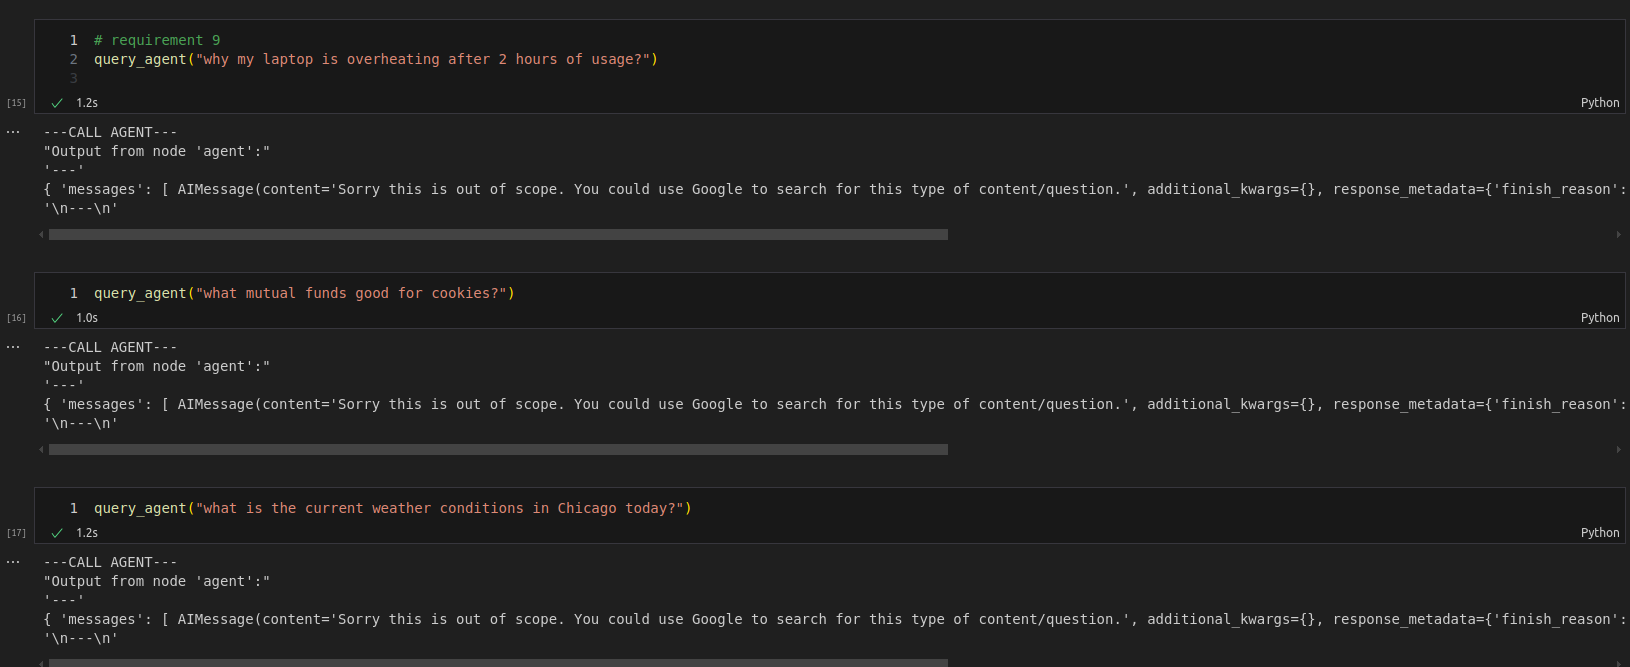
\includegraphics[height=175pt]{req_9.png}
\end{center}

The agent also responded appropriately to the `greeting-like' prompt:

\begin{center}
    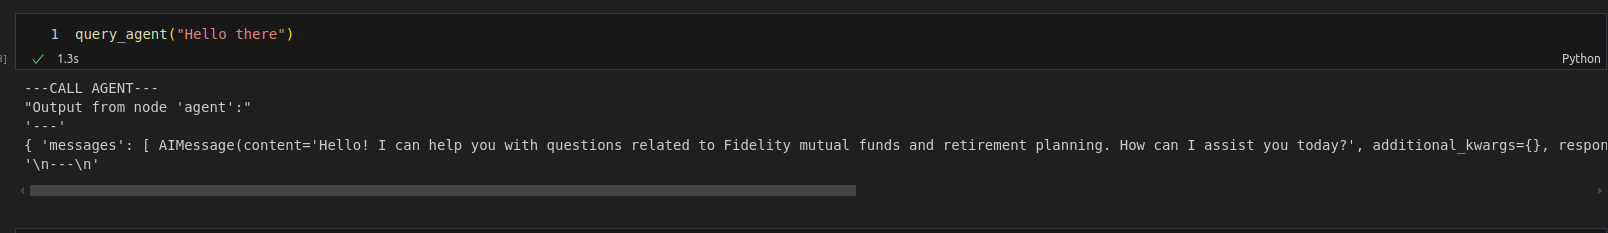
\includegraphics{req_9B.png}
\end{center}

Cells 10-20 show the queries made to the agent graph. Relevant prompts are answered with quality responses.
Irrelevant prompts are flagged out of scope. The question about Fidelity specific funds are answered and the 
prompt about Schwab funds are correctly identified as out of scope.

\clearpage

\section*{Requirement 10: Load a PDF into context}
\tab In cell 21 the \textit{FFFGX.pdf} document is loaded using the \textbf{PyPDFLoader}. In cell 22 we view the meta data and content.
In cell 23 the document is added to the ChromaDB vector store. Finally, in cells 24 and 25 we display a graphic representation of what
was processed.

\section*{Requirement 11: Test the context with queries}
\tab In cell 26 I construct a function, \textbf{query\_llm}, that can be used to query an OpenAI chat client in a DRY manner.
Cells 27-30 show the prompts and responses. The LLM, using the PDF context, was able to answer questions from the text and tables
of the document. Very impressive libraries on display here!

\begin{center}
    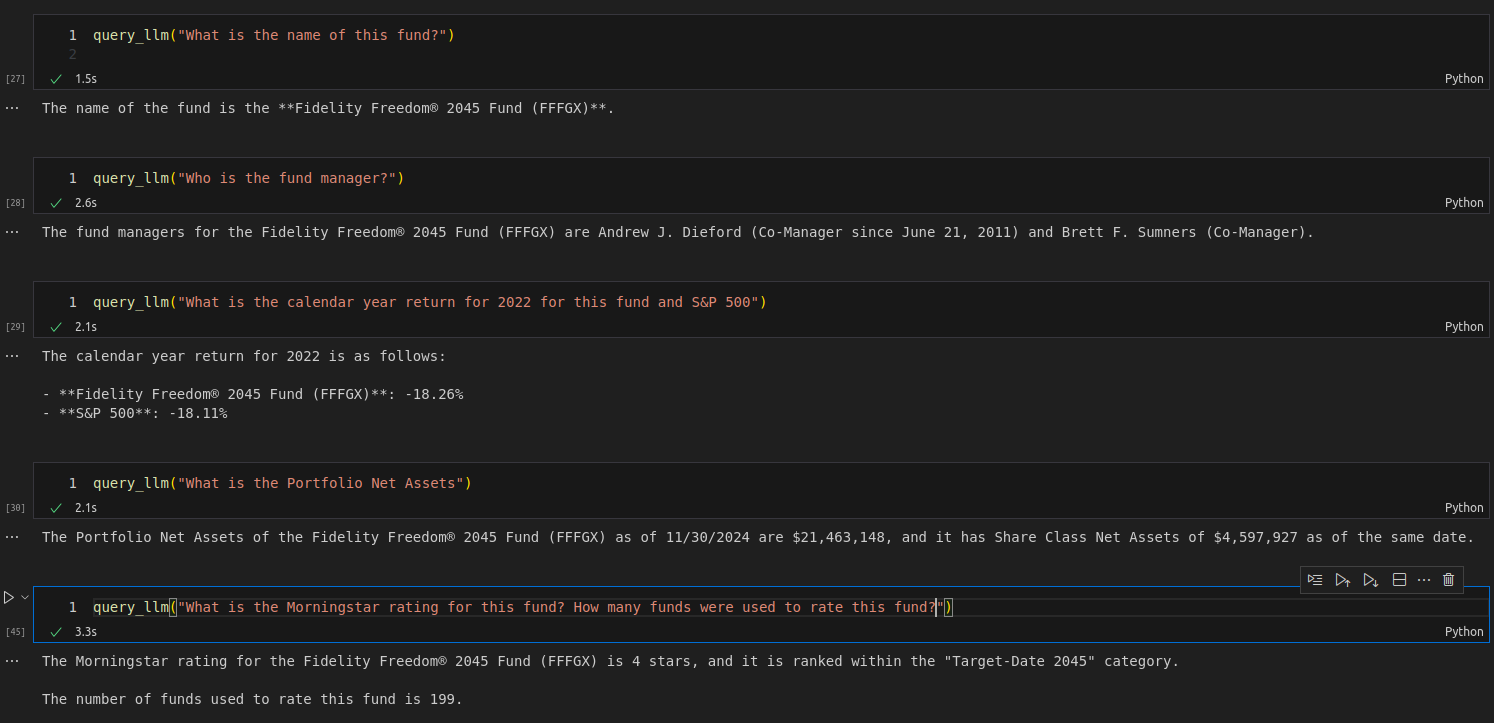
\includegraphics{req_11.png}
\end{center}


\end{document}